\section{Evaluating Off-the-Shelf Models for Tool-Call Speculation}
\label{sec:empirical-self-speculate}

Off-the-shelf draft models are a natural starting point for tool-call speculation. We
evaluate their speculator--agent gap in realistic agentic settings, where the
speculator observes the deployed agent's context immediately before a tool call
and predicts the next tool call, including both the tool name and
arguments. This setup measures whether an off-the-shelf model can match the
deployed agent's tool decisions under the same inference-time context.

\subsection{Evaluation Protocol}
\label{sec:empirical-self-speculate:protocol}

For each target agent, we run speculation online during the agent's rollout. 
In each domain, we sample 50 evaluation queries and execute the deployed agent in the environment. 
Whenever the rollout reaches a tool-call boundary, the serving controller switches from the target
agent model to an off-the-shelf speculator model. 
The speculator receives the current trajectory prefix with a fixed speculation suffix appended:
\begin{quote}
\small\ttfamily
\textless think\textgreater{} Okay, let's see. The user provided what I need.
I'll look it up. The next step is to make the tool call.
\textless/think\textgreater{}
\end{quote}
The speculator then decodes one candidate tool call. The controller switches
back to the target agent, lets the agent produce the actual call, and executes
the agent's call in the environment. Thus speculation is evaluated under the
same online state that the agent sees, while the environment state is still
determined only by the deployed agent.
Figure~\ref{fig:speculation-rollout-example} illustrates this online comparison in a
$\tau$-bench trajectory: the speculator is prompted from the current prefix, the
agent continues independently, and the pre-executed result is reusable only when
the speculated tool name and arguments exactly match the agent's eventual call.

\begin{figure}[t]
\centering
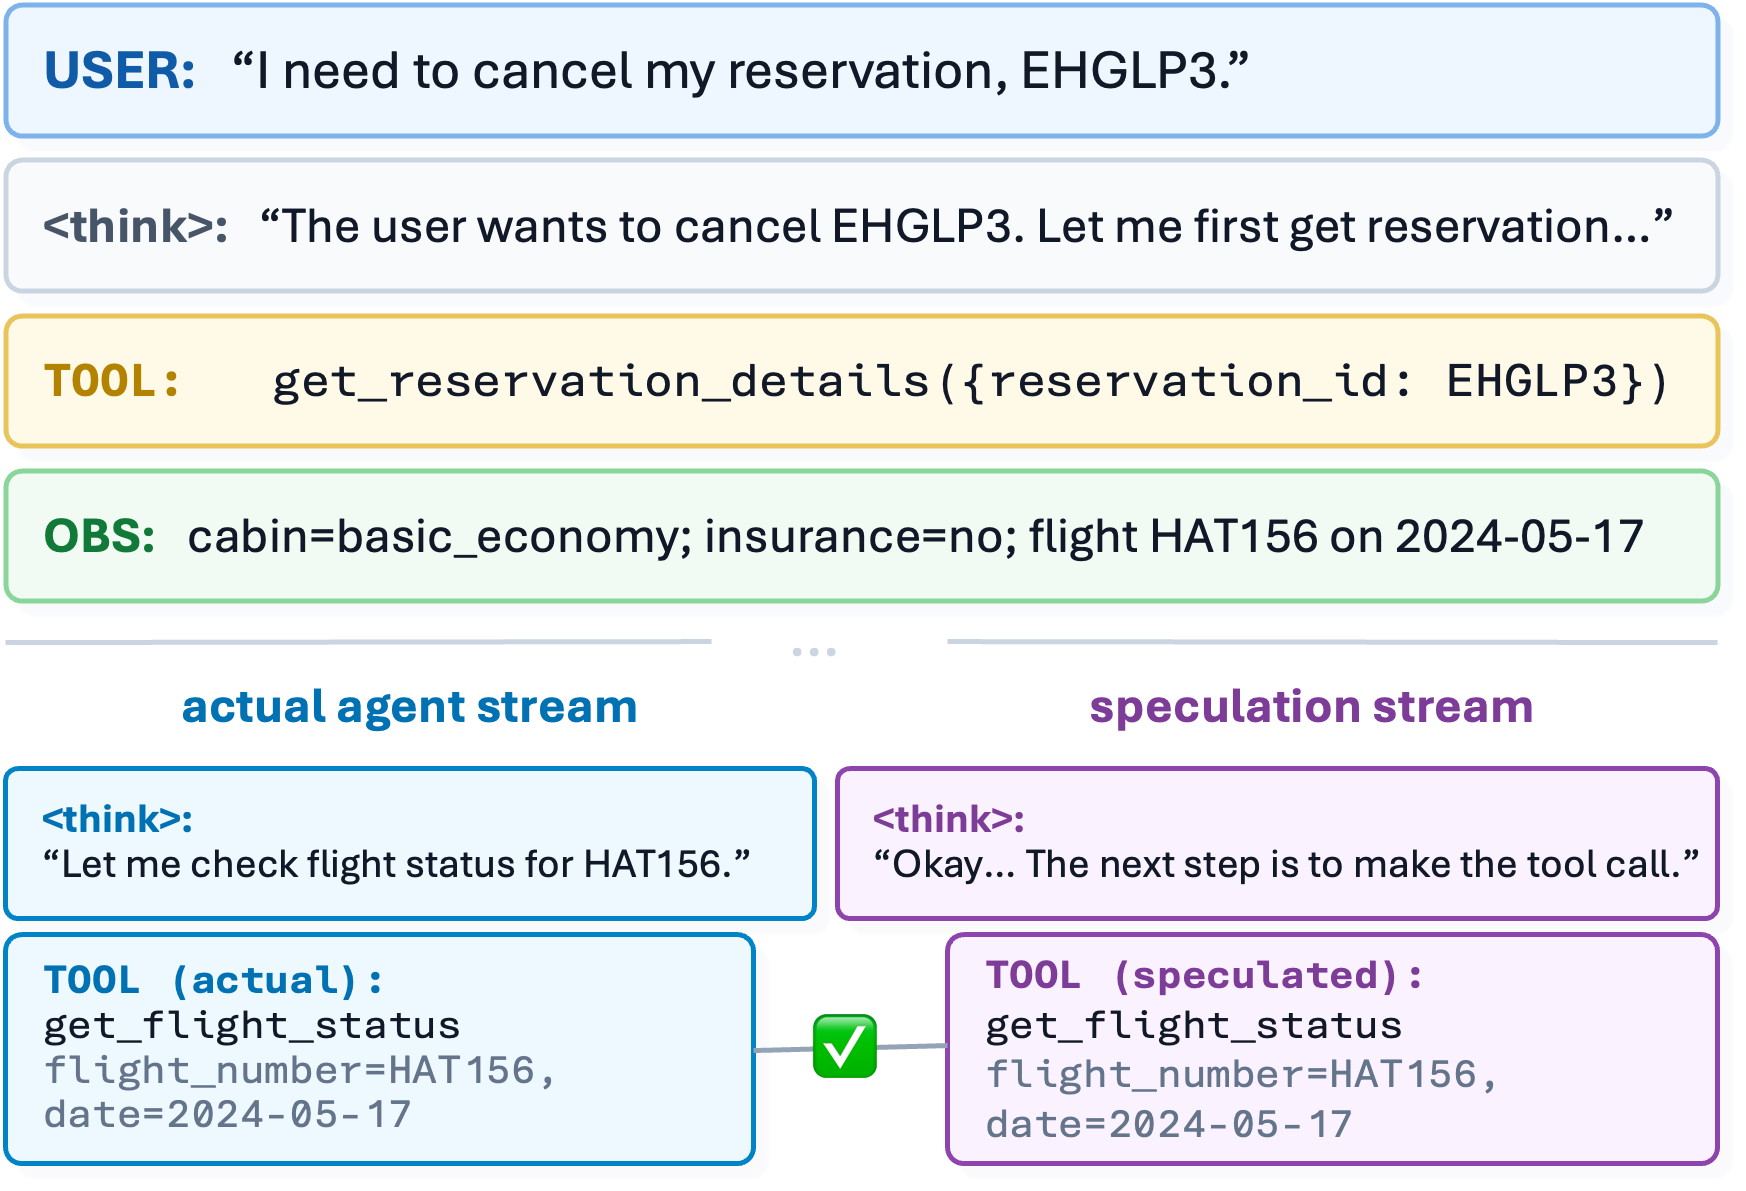
\includegraphics[width=0.92\linewidth]{figures/example-speculation.png}
\vspace{1mm}
\caption{Online tool-call speculation example. From the shared trajectory
prefix, the left stream continues to the agent's reasoning and actual tool call generation, while the
right stream predicts the tool call in parallel. 
% The result is reusable only when
% the tool name and arguments match exactly.
}
\label{fig:speculation-rollout-example}
\vspace*{-0.12in}
\end{figure}

We instantiate this protocol in two same-family comparisons. For Qwen3-4B agent, we
evaluate Qwen3-0.6B and Qwen3-1.7B as speculators; for Qwen3.5-4B agent, we
evaluate Qwen3.5-0.8B and Qwen3.5-2B. In both families, we also prompt the
target 4B model to predict its own next call from the same online prefix. 
We run the protocol on 50 queries from MuSiQue in the agentic SearchQA environment~\citep{jin2025searchr1} and airline domain of $\tau$-bench~\citep{yao2024taubench,barres2025tau2bench}.

Table~\ref{tab:offshelf-results} reports both prediction quality and serving
cost. We use Hit@1 exact match as the primary speculation metric because a
pre-executed tool call is reusable only when both the tool name and argument
dictionary match the agent's eventual call. We also report speculation
wall-clock time and peak GPU memory to capture the overhead of alternating
between the target agent and a separate draft model during the same rollout. The
memory estimate includes both resident model weights and peak KV-cache state:
external speculators require the target agent weights, the draft model weights,
and two active KV caches, whereas self-speculation reuses the target model
weights and the target prefix KV cache, adding only the small speculation branch.
All measurements in this off-the-shelf setting use a single H100 GPU. We
implement the comparison in the SGLang inference engine with an explicit
parameter switch between the external drafter model and the target agent model,
so each query serially alternates agent generation, speculator generation, and
agent continuation while recording time and memory usage.

\begin{table}[t]
\centering
\renewcommand{\arraystretch}{1.1}
\small
\setlength{\tabcolsep}{2.5pt}
\resizebox{0.95\columnwidth}{!}{%
\begin{tabular}{@{}l|ccc|ccc@{}}
\toprule \midrule
\multirow{2}{*}{Speculator} &
\multicolumn{3}{c|}{\textbf{MuSiQue}} &
\multicolumn{3}{c}{\textbf{$\tau$-bench}} \\
\cmidrule(lr){2-4} \cmidrule(lr){5-7}
 & H@1$\uparrow$ & Time$\downarrow$ & Mem.$\downarrow$
 & H@1$\uparrow$ & Time$\downarrow$ & Mem.$\downarrow$ \\
\midrule
\rowcolor{transgray}
\multicolumn{7}{c}{\textbf{Target agent: Qwen3-4B}} \\
\midrule
Qwen3-0.6B & 4.3 & 27.4 & 10.71 & 16.8 & 45.2 & 14.59 \\
Qwen3-1.7B & 14.7 & 33.1 & 12.76 & 25.4 & 52.1 & 16.64 \\
Qwen3-4B self & \textbf{25.3} & \textbf{8.3} & \textbf{8.70} & \textbf{37.2} & \textbf{24.1} & \textbf{10.90} \\
\midrule
\rowcolor{transgray}
\multicolumn{7}{c}{\textbf{Target agent: Qwen3.5-4B}} \\
\midrule
Qwen3.5-0.8B & 8.7 & 22.3 & 9.31 & 21.3 & 39.2 & 9.98 \\
Qwen3.5-2B & 16.2 & 30.6 & 11.55 & 32.8 & 54.1 & 12.22 \\
Qwen3.5-4B self & \textbf{27.4} & \textbf{6.7} & \textbf{7.73} & \textbf{44.1} & \textbf{19.1} & \textbf{8.22} \\
\midrule
\bottomrule
\end{tabular}
}
\caption{Online off-the-shelf speculation results. For each target 4B agent, we
compare smaller same-family external draft speculators with the target model
prompted to speculate its own next tool call. GPU memory includes model weights
and peak KV-cache.}
\label{tab:offshelf-results}
\vspace*{-0.12in}
\end{table}


\subsection{Findings}
\label{sec:empirical-self-speculate:findings}

\paragraph{External speculators add serving overhead.} Even small draft models
require additional weights and a second KV cache, so their cost is not just the
extra decoding step. In Table~\ref{tab:offshelf-results}, Qwen3-4B on MuSiQue
increases from 8.70GB and 8.3s with self-speculation to 10.71GB/27.4s with
Qwen3-0.6B and 12.76GB/33.1s with Qwen3-1.7B. The same pattern appears in
$\tau$-bench and in the Qwen3.5 series. External speculation therefore needs
large Hit@1 gains to justify the extra serving cost, especially when memory is
limited or agentic contexts are long.

\paragraph{The agent is the strongest off-the-shelf speculator for itself.} The
target agent outperforms smaller same-family draft models, indicating that
family similarity alone does not recover the target agent's next-call
distribution. For Qwen3-4B, self-speculation reaches 25.3 Hit@1 on MuSiQue and
37.2 on $\tau$-bench, compared with 14.7 and 25.4 for the strongest external
speculator. For Qwen3.5-4B, self-speculation improves over Qwen3.5-2B from 16.2
to 27.4 on MuSiQue and from 32.8 to 44.1 on $\tau$-bench. This supports the
speculator--agent gap: the best off-the-shelf predictor of an agent's next call
is often the agent itself. These findings motivate training the agent itself as
the speculator instead of deploying a separate external LLM.
